\documentclass[11pt,letterpaper]{article}
\usepackage[lmargin=1in,rmargin=1in,bmargin=1in,tmargin=1in]{geometry}
\usepackage{style/quiz}
\usepackage{style/commands}

% -------------------
% Content
% -------------------
\begin{document}
\thispagestyle{title}

% Quiz 1
\quizsol \textit{True/False}: If $a$ and $b$ are distinct primes, then $\gcd(a, b)= 1$. \pspace

\sol The statement is \textit{true}. Because $a$ is prime, the only divisors of $a$ are 1 and $a$. But then if $a$ and $b$ are distinct primes, then $a \neq b$. But then the only common divisor for $a$ and $b$ is 1. Therefore, $\gcd(a, b)= 1$. For instance, if $a= 3$ and $b= 5$, we have $\gcd(a, b)= \gcd(3, 5)= 1$. \pvspace{1.3cm}



% Quiz 2
\quizsol \textit{True/False}: There is a rational number equal to the following decimal:
	\[
	0.123456789101112131415\ldots
	\]

\sol The statement is \textit{false}. A rational number is a real number, i.e. decimal number, whose decimal expansion either terminates or repeats. The decimal number above simply `counts out' all the integers. Observe that the decimal expansion is 1, 2, 3, 4, \dots. But then the decimal expansion does not terminate nor does it repeat. Therefore, the decimal number above cannot be rational. \pvspace{1.3cm}



% Quiz 3
\quizsol \textit{True/False}: $\sqrt[4]{2^{100} \cdot 3^{21} \cdot 5^{42}}= 2^{25} \cdot 3^5 \cdot 5^{10} \sqrt[4]{3^1 \cdot 5^2}$ \pspace

\sol The statement is \textit{true}. We have\dots
	\[
	\sqrt[4]{2^{100} \cdot 3^{21} \cdot 5^{42}}= \sqrt[4]{2^{100} \cdot (3^{20} \cdot 3^1) \cdot (5^{40} \cdot 5^2)}= 2^{100/4} \cdot 3^{20/4} \cdot 5^{40/4} \sqrt[4]{3^1 \cdot 5^2}= 2^{25} \cdot 3^5 \cdot 5^{10} \sqrt[4]{3^1 \cdot 5^2}
	\]
Alternatively, observe\dots
	\[
	\sqrt[4]{2^{100} \cdot 3^{21} \cdot 5^{42}}= (2^{100} \cdot 3^{21} \cdot 5^{42})^{1/4}= 2^{25} \cdot 3^{4 + 1/4} \cdot 5^{10 + 2/4}= 2^{25} \cdot 3^4 \cdot 5^{10} \sqrt[4]{3^1 \cdot 5^2}
	\] \pvspace{1.3cm}



% Quiz 4
\quizsol \textit{True/False}: In a course, the first exam is worth 15\% of your course grade. If you receives an 80\% on that exam, then your maximum possible course grade is a 88\%. \pspace

\sol The statement is \textit{false}. Because you received an 80\%, you only received 80\% of the 15~total points possible. Therefore, you have earned $15(0.80)= 12$ points toward your average. But then you have lost $15 - 12= 3$ of your course grade. Therefore, your maximum possible grade is $100 - 3= 97$. Alternatively, by receiving an 80\%, you have lost $100\% - 80\%= 20\%$ of the 15~points of your course grade. Therefore, you have lost $15(0.20)= 3$ points of your overall average. Therefore, your maximum possible course grade is $100 - 3= 97$. \pvspace{1.3cm}



% Quiz 5
\quizsol \textit{True/False}: A function can have more than one $y$-intercept. \pspace

\sol The statement is \textit{false}. Suppose the function had more than one $y$-intercept. Say $A$ and $B$ are $y$-intercepts, i.e. $(0, A)$ and $(0, B)$ are $y$-intercepts. But then the vertical line at $x= 0$ intersects the graph of the function in at least two points---namely, $(0, A)$ and $(0, B)$. But then the function fails the vertical line test. Therefore, the `function' cannot actually be a function. Alternatively, Say $A$ and $B$ are $y$-intercepts, i.e. $(0, A)$ and $(0, B)$ are $y$-intercepts. But then the `function' is not well defined at $x= 0$. Therefore, the `function' is not actually a function. \pvspace{1.3cm}



% Quiz 6
\quizsol \textit{True/False}: If $f(x)= 6x - 5$ and $f^{-1}(x)$ exists, then $f^{-1}(3)= 13$. \pspace

\sol The statement is \textit{false}. Recall that if $f^{-1}(y)= x$, then $f(x)= y$. So if $f^{-1}(3)= 13$, then $f(13)= 3$. However, $f(13)= 6(13) - 5= 78 - 5= 73 \neq 3$. We can even find the correct value. Suppose that $x= f^{-1}(3)$. Then we have\dots
	\[
	\begin{aligned}
	x&= f^{-1}(3) \\
	f(x)&= f(f^{-1}(3)) \\
	f(x)&= 3 \\
	6x - 5&= 3 \\
	6x&= 8 \\
	x&= \dfrac{8}{6} \\
	x&= \dfrac{4}{3}
	\end{aligned}
	\]
We can check this as $f(\frac{4}{3})= 6 \cdot \frac{4}{3} - 5= 8 - 5= 3$. Therefore, $f^{-1}(3)= \frac{4}{3}$. \pvspace{1.5cm}



% Quiz 7
\quizsol \textit{True/False}: Corn syrup is flowing into a large storage vat in a beverage processing plant at a roughly constant rate. These vats can hold 500~gallons of liquid and the vats are currently holding 75~gallons of syrup. The amount of volume remaining unfilled in the vat is a linear function of time. \pspace

\sol The statement is \textit{true}. A linear function has a constant rate of change. Vice versa, if something is changing at a (roughly) constant rate, it should be (roughly) linear. Because the corn syrup is flowing into the vats at a constant rate, the amount of volume remaining in the vats is decreasing at the same constant rate. Therefore, the amount of unfilled volume in the vats is approximately linear. In fact, we can find this as a linear function in time. Let $V(t)$ denote the volume remaining in the vats at time $t$. We know vats currently ($t= 0$) hold 75~gallons of syrup. Therefore, they have a remaining volume of $500 - 75= 425$~gallons, i.e. $V(0)= 425$. Let $r$ be the rate at which syrup is flowing into the vats. Then the rate of change of the volume remaining in the vats is $-r$ (because the volume is decreasing). Because $V(t)$ is linear, we know that $V(t)= mt + b$. But then $V(t)= -rt + b$. Finally, using the fact that $V(0)= 425$, we have $425= -r(0) + b$ so that $b= 425$. Therefore, $V(t)= 425 - rt$. \pvspace{1.3cm}



\newpage



% Quiz 8
\quizsol \textit{True/False}: If $x - 7 \sqrt{2}= \dfrac{\pi x + 9}{\sqrt{2}}$, then $x= \dfrac{-23}{\pi - \sqrt{2}}$. \pspace

\sol The statement is \textit{true}. We have\dots
	\[
	\begin{aligned}
	x - 7 \sqrt{2}&= \dfrac{\pi x + 9}{\sqrt{2}} \\
	\sqrt{2} (x - 7\sqrt{2})&= \dfrac{\pi x + 9}{\sqrt{2}} \cdot \sqrt{2} \\
	\sqrt{2}x - 7 \cdot 2&= \pi x + 9 \\
	\sqrt{2}x - 14&= \pi x + 9 \\
	-23&= \pi x - \sqrt{2} x \\
	(\pi - \sqrt{2})x&= -23 \\
	x&= \dfrac{-23}{\pi - \sqrt{2}}
	\end{aligned}
	\]
Equivalently, 
	\[
	\begin{aligned}
	x - 7 \sqrt{2}&= \dfrac{\pi x + 9}{\sqrt{2}} \\
	\sqrt{2} (x - 7\sqrt{2})&= \dfrac{\pi x + 9}{\sqrt{2}} \cdot \sqrt{2} \\
	\sqrt{2}x - 7 \cdot 2&= \pi x + 9 \\
	\sqrt{2}x - \pi x&= 23 \\
	(\sqrt{2} - \pi) x&= 23 \\
	x&= \dfrac{23}{\sqrt{2} - \pi}
	\end{aligned}
	\]
To see that this is equivalent to the given answer, observe
	\[
	\dfrac{23}{\sqrt{2} - \pi}= \dfrac{23}{\sqrt{2} - \pi} \cdot \dfrac{-1}{-1}= \dfrac{-23}{-(\sqrt{2} - \pi)}= \dfrac{-23}{\pi - \sqrt{2}}
	\] \pvspace{1.5cm}



% Quiz 9
\quizsol \textit{True/False}: The function $f(x)= 10 - 2(x + 1)^2$ is a parabola that is concave up with vertex $(-1, 10)$. \pspace

\sol The statement is \textit{false}. The vertex form of a quadratic function $ax^2 + bx + c$ is $y= a(x - P)^2 + Q$, where $(P, Q)$ is the vertex of the quadratic function. We have
	\[
	f(x)= 10 - 2(x + 1)^2= -2(x + 1)^2 + 10= -2 \big(x - (-1) \big)^2 + 10
	\]
But then $a= -2$, and $(P, Q)= (-1, 10)$. Therefore, the vertex is $(-1, 10)$, but because $a= -2 < 0$, the quadratic function is concave down. 



\newpage



% Quiz 10
\quizsol \textit{True/False}: The function $f(x)= x^2 - 4x + 5$ does not factor `nicely' over the reals but does factor `nicely' over the complex numbers. \pspace

\sol The statement is \textit{true}. A quadratic function $ax^2 + bx + c$ factors `nicely' if and only if the absolute value of the discriminant, $|D|= |b^2 - 4ac|$, is a perfect square. If $D \geq 0$, then it factors `nicely' over the reals, and if $D < 0$, then it only factors `nicely' over the complex numbers. We have $a= 1$, $b= -4$, $c= 5$. Then $D= (-4)^2 - 4(1)5= 16 - 20= -4$. Because $|D|= |-4|= 4$ is a perfect square and $D < 0$, $f(x)$ factors `nicely' but only over the complex numbers. \pvspace{1.5cm}



% Quiz 11
\quizsol \textit{True/False}: The polynomial $x^2 + x + 1$ can be factored as\dots
	\[
	\left( x - \left( \dfrac{1 - \sqrt{3}\,i}{2} \right) \right) \left( x - \left( \dfrac{1 + \sqrt{3}\,i}{2} \right) \right)
	\] \pspace

\sol The statement is \textit{true}. If a quadratic function $f(x)= ax^2 + bx + c$ has roots $r_1$ and $r_2$, then $f(x)$ factors as $f(x)= a(x - r_1)(x - r_2)$. The roots of $f(x)$ are the solutions to $f(x)= 0$, which we can always find using the quadratic formula. Solving the equation $x^2 + x + 1= 0$ using the quadratic formula with $a= 1$, $b= 1$, and $c= 1$, we have\dots
	\[
	\begin{aligned}
	x&= \dfrac{-b \pm \sqrt{b^2 - 4ac}}{2a} \\[0.3cm]
	&= \dfrac{-1 \pm \sqrt{1^2 - 4(1)1}}{2(1)} \\[0.3cm]
	&= \dfrac{-1 \pm \sqrt{1 - 4}}{2} \\[0.3cm]
	&= \dfrac{-1 \pm \sqrt{-3}}{2} \\[0.3cm]
	&= \dfrac{-1 \pm \sqrt{3}\,i}{2}
	\end{aligned}
	\]
But then $f(x)$ factors as\dots
	\[
	\begin{aligned}
	f(x)&= a(x - r_1)(x - r_2) \\[0.3cm]
	&= 1 \cdot \left( x - \left( \dfrac{1 - \sqrt{3}\,i}{2} \right) \right) \left( x - \left( \dfrac{1 + \sqrt{3}\,i}{2} \right) \right) \\[0.3cm]
	&= \left( x - \left( \dfrac{1 - \sqrt{3}\,i}{2} \right) \right) \left( x - \left( \dfrac{1 + \sqrt{3}\,i}{2} \right) \right)
	\end{aligned}
	\]



% Quiz 13
\quizsol \textit{True/False}: There are 5 solutions to the system of equations given by the curves below:
	\[
	\fbox{
	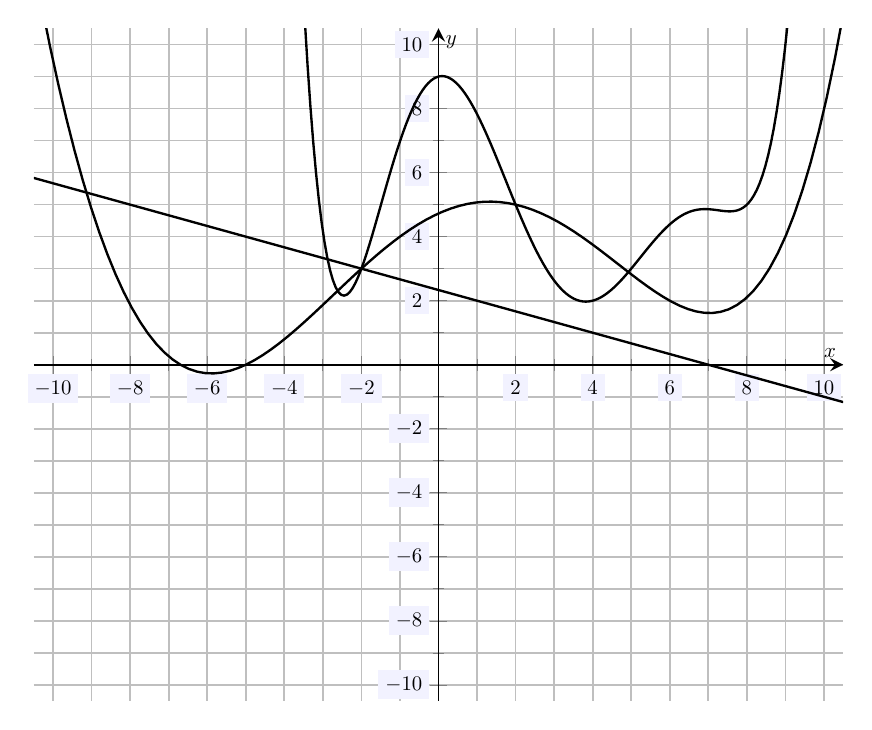
\begin{tikzpicture}[scale=1.5,every node/.style={scale=0.5}]
	\begin{axis}[
	grid=both,
	axis lines=middle,
	ticklabel style={fill=blue!5!white},
	xmin= -10.5, xmax=10.5,
	ymin= -10.5, ymax=10.5,
	xtick={-10,-8,-6,-4,-2,0,2,4,6,8,10},
	ytick={-10,-8,-6,-4,-2,0,2,4,6,8,10},
	minor tick = {-10,-9,...,10},
	xlabel=\(x\),ylabel=\(y\),
	]
%	\draw[fill=black] (-6,4) circle (0.05cm);
	\addplot[line width= 0.02cm,domain= -10.5:10.5] ({x},{2.3333 - 0.3333*x}); 
	\addplot[line width= 0.02cm,domain= -5:9.5,samples=200] ({x},{9. + 0.313709*x - 1.71066*x^2 + 0.134488*x^3 + 0.110565*x^4 -  0.0219787*x^5 + 0.00114989*x^6}); 
	\addplot[line width= 0.02cm,domain= -10.5:10.5,samples=100] ({x},{4.72287 + 0.547233*x - 0.189916*x^2 - 0.01204*x^3 + 0.00229978*x^4 + 0.0000579777*x^5}); 
	\end{axis}
	\end{tikzpicture}
	}
	\] \pspace

\sol The statement is \textit{false}. There are five points where any two or more of the curves intersect---given by the black points in the figure below. However, for a point to be a solution to the system of equations given by the curves, it must lie on \textit{all} the curves simultaneously. There is only one point that lies on all the curves---the red point shown in the figure below. Therefore, there is only one solution to the system of equations given by the curves. 
	\[
	\fbox{
	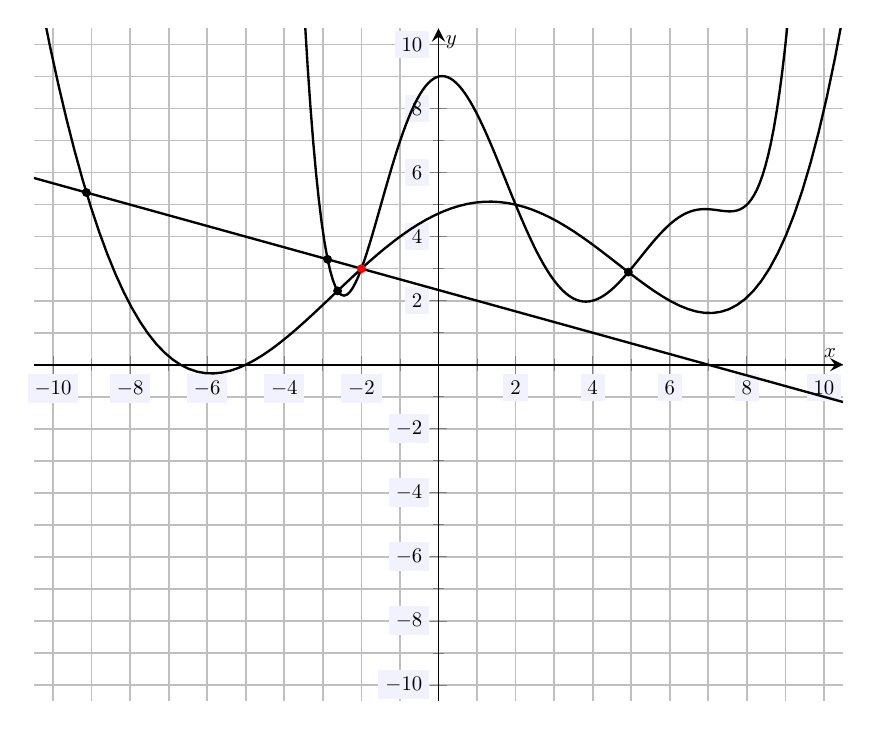
\begin{tikzpicture}[scale=1.5,every node/.style={scale=0.5}]
	\begin{axis}[
	grid=both,
	axis lines=middle,
	ticklabel style={fill=blue!5!white},
	xmin= -10.5, xmax=10.5,
	ymin= -10.5, ymax=10.5,
	xtick={-10,-8,-6,-4,-2,0,2,4,6,8,10},
	ytick={-10,-8,-6,-4,-2,0,2,4,6,8,10},
	minor tick = {-10,-9,...,10},
	xlabel=\(x\),ylabel=\(y\),
	]
%	\draw[fill=black] (-6,4) circle (0.05cm);
	\addplot[line width= 0.02cm,domain= -10.5:10.5] ({x},{2.3333 - 0.3333*x}); 
	\addplot[line width= 0.02cm,domain= -5:9.5,samples=200] ({x},{9. + 0.313709*x - 1.71066*x^2 + 0.134488*x^3 + 0.110565*x^4 -  0.0219787*x^5 + 0.00114989*x^6}); 
	\addplot[line width= 0.02cm,domain= -10.5:10.5,samples=100] ({x},{4.72287 + 0.547233*x - 0.189916*x^2 - 0.01204*x^3 + 0.00229978*x^4 + 0.0000579777*x^5}); 
	\draw[fill=black] (-9.13432,5.37778) circle (0.03cm);
	\draw[fill=black] (-2.617186,2.30642) circle (0.03cm);
	\draw[fill=black] (-2.8766,3.29206) circle (0.03cm);
	\draw[red,fill=red] (-2,3) circle (0.03cm);
	\draw[fill=black] (4.92594,2.89334) circle (0.03cm);
	\end{axis}
	\end{tikzpicture}
	}
	\] 



\newpage



% Quiz 13
\quizsol \textit{True/False}: When $f(x)= 4(5^{1 - 2x})$ is expressed in the form $y= Ab^x$, we have $f(x)= 20 \left( \dfrac{1}{25} \right)^x$. \pspace

\sol The statement is \textit{true}. We have\dots
	\[
	f(x)= 4(5^{1 - 2x})= 4 \cdot (5^1 \cdot 5^{-2x})= 20 \cdot 5^{-2x}= 20 (5^{-2})^x= 20 \left( \dfrac{1}{25} \right)^x
	\] \pvspace{1.3cm}



% Quiz 14
\quizsol \textit{True/False}: If Luke invests \$650 in a savings account that earns 8.2\% yearly annual interest, compounded monthly, then the amount he has after 6 years is\dots
	\[
	650 \left( 1 + \dfrac{0.082}{12} \right)^6
	\]

\sol The statement is \textit{false}. If a principal $P$ is invested at an annual interest rate $r$, compounded $k$ times per year for $t$ years, then the amount of money is given by
	\[
	P \left(1 + \dfrac{r}{k} \right)^{kt}
	\]
Here, we have $P= 650$, $r= 0.082$, $k= 12$, and $t= 6$. But then the amount of money is given by\dots
	\[
	P \left(1 + \dfrac{r}{k} \right)^{kt}= 650 \left(1 + \dfrac{0.082}{12} \right)^{12 \cdot 6}
	\] \pvspace{1.3cm}



% Quiz 15
\quizsol \textit{True/False}: Written as a single logarithm, then
	\[
	\dfrac{1}{3}\, \log_5(x) - 7\log_5(y) - 2= \log_5 \left( \dfrac{\sqrt[3]{x}}{25y^7} \right)
	\]

\sol The statement is \textit{true}. We have\dots
	\[
	\begin{aligned}
	\dfrac{1}{3}\, \log_5(x) - 7\log_5(y) - 2&= \dfrac{1}{3}\, \log_5(x) - 7\log_5(y) - \log_5(5^2) \\
	&= \log_5(\sqrt[3]{x}) - \log_5(y^7) - \log_5(25) \\
	&= \log_5 \left( \dfrac{\sqrt[3]{x}}{25y^7} \right)
	\end{aligned}
	\] \vfill



% Quiz 16
\quizsol \textit{True/False}: There are 10,560 digits in $1250^{3410}$. \pspace

\sol The statement is \textit{false}. We know that the number of digits in a number $N$ is the smallest integer that is greater than $\log_{10} N$. We have $\log_{10}(1250^{3410})= 3410 \log_{10}(1250) \approx 10560.463$. The smallest integer that is greater than this number is 10561. Therefore, $125^{341}$ has 10,561 digits. 


\end{document}